\documentclass[aspectratio=169, xcolor=dvipsnames]{beamer}

% --- Theme Setup ---
\usetheme{Madrid}
\usecolortheme{default}

% --- Packages ---
\usepackage{graphicx}
\usepackage{xcolor}
\usepackage{booktabs}
\usepackage{hyperref}
\usepackage{adjustbox}
\usepackage{amssymb}
\usepackage{longtable}
\usepackage{caption}

% --- Title Information ---
\title{Module 06}
\subtitle{Introduction to Relational Model/1}
\author{Milav Dabgar}
\institute{www.milav.in}
\date{\today}

\begin{document}

% Title Slide
\begin{frame}
    \titlepage
\end{frame}

\begin{frame}{Week Recap}
    \begin{itemize}
        \item The proliferation of DBMS in wide range of applications provide motivation to study the subject
        \item Know Your Course provided information about prerequisites, outline and text book
        \item The specific need for a DBMS discussed in contrast to a file system based application using a programming language like Python
        \item Basic notions of a DBMS are introduced
    \end{itemize}
\end{frame}

\begin{frame}{Module Objectives}
    \begin{itemize}
        \item To understand attributes and their types
        \item To understand the mathematical structure of relational model
        \begin{itemize}
            \item Schema
            \item Instance
            \item Keys
        \end{itemize}
        \item To familiarize with different types of relational query languages
    \end{itemize}
\end{frame}

\begin{frame}{Module Outline}
    \begin{itemize}
        \item Attribute Types
        \item Relation Schema and Instance
        \item Keys
        \item Relational Query Languages
    \end{itemize}
\end{frame}

\section{Example of a Relation}

\begin{frame}
  \vfill
  \centering
  \begin{beamercolorbox}[sep=8pt,center,shadow=true,rounded=true]{title}
    \usebeamerfont{title}Example of a Relation\par%
  \end{beamercolorbox}
  \vfill
\end{frame}

\begin{frame}{Example of a Relation}
    \begin{center}
        \begin{adjustbox}{max width=\textwidth}
        \begin{tabular}{|l|l|l|l|}
        \hline
        \textbf{ID} & \textbf{name} & \textbf{dept\_name} & \textbf{salary} \\ \hline
        10101 & Srinivasan & Comp. Sci. & 65000 \\ \hline
        12121 & Wu         & Finance    & 90000 \\ \hline
        15151 & Mozart     & Music      & 40000 \\ \hline
        22222 & Einstein   & Physics    & 95000 \\ \hline
        45565 & El Said    & History    & 60000 \\ \hline
        58583 & Gold       & Physics    & 87000 \\ \hline
        76543 & Katz       & Comp. Sci. & 75000 \\ \hline
        76766 & Califieri  & History    & 62000 \\ \hline
        83821 & Singh      & Finance    & 80000 \\ \hline
        98345 & Crick      & Biology    & 72000 \\ \hline
        \dots & \dots      & \dots      & \dots \\ \hline
        \end{tabular}
        \end{adjustbox}
        
        \vspace{1em}
        \textit{Columns are attributes; rows are tuples.}
    \end{center}
\end{frame}

\section{Attributes}

\begin{frame}
  \vfill
  \centering
  \begin{beamercolorbox}[sep=8pt,center,shadow=true,rounded=true]{title}
    \usebeamerfont{title}Attributes\par%
  \end{beamercolorbox}
  \vfill
\end{frame}

\begin{frame}{Attribute Types}
    \begin{itemize}
        \item Consider \texttt{Students = (Roll\#, First Name, Last Name, DoB, Passport\#, Aadhaar\#, Department)} relation
        \item The set of allowed values for each attribute is called the \textbf{domain} of the attribute
        \begin{itemize}
            \item \textbf{Roll\#}: Alphanumeric string
            \item \textbf{First Name, Last Name}: Alpha String
            \item \textbf{DoB}: Date
            \item \textbf{Passport\#}: String (Letter followed by 7 digits) - nullable (optional)
            \item \textbf{Aadhaar\#}: 12-digit number
            \item \textbf{Department}: Alpha String
        \end{itemize}
        \item Attribute values are (normally) required to be \textbf{atomic}; that is, indivisible
        \item The special value \textbf{null} is a member of every domain. Indicates that the value is unknown
        \item The null value may cause complications in the definition of many operations
    \end{itemize}
\end{frame}

\begin{frame}{Attribute Types (2)}
    \begin{center}
        \begin{adjustbox}{max width=\textwidth}
        \begin{tabular}{|l|l|l|l|l|l|l|}
        \hline
        \textbf{Roll \#} & \textbf{First Name} & \textbf{Last Name} & \textbf{DoB} & \textbf{Passport \#} & \textbf{Aadhaar \#} & \textbf{Department} \\ \hline
        15CS10026 & Lalit & Dubey & 27-Mar-1997 & L4032464 & 1728-6174-9239 & Computer \\ \hline
        16EE30029 & Jatin & Chopra & 17-Nov-1996 & \textit{null} & 3917-1836-3816 & Electrical \\ \hline
        \end{tabular}
        \end{adjustbox}
    \end{center}
\end{frame}

\section{Schema and Instance}

\begin{frame}
  \vfill
  \centering
  \begin{beamercolorbox}[sep=8pt,center,shadow=true,rounded=true]{title}
    \usebeamerfont{title}Schema and Instance\par%
  \end{beamercolorbox}
  \vfill
\end{frame}

\begin{frame}{Relation Schema and Instance}
    \begin{itemize}
        \item $A_1, A_2, \dots, A_n$ are attributes
        \item $R = (A_1, A_2, \dots, A_n)$ is a \textbf{relation schema}. Example: \texttt{instructor = (ID, name, dept\_name, salary)}
        \item Formally, given sets $D_1, D_2, \dots, D_n$ a \textbf{relation} $r$ is a subset of $D_1 \times D_2 \times \dots \times D_n$.
        \item Thus, a relation is a set of $n$-tuples $(a_1, a_2, \dots, a_n)$ where each $a_i \in D_i$
        \item The current values (\textbf{relation instance}) of a relation are specified by a table
        \item An element $t$ of $r$ is a \textbf{tuple}, represented by a row in a table
        \item Example: $\text{instructor} \subseteq (\text{String(5)} \times \text{String} \times \text{String} \times \text{Number}^+)$, where \texttt{ID} $\in \text{String(5)}$, \texttt{name} $\in \text{String}$, \texttt{dept\_name} $\in \text{String}$, and \texttt{salary} $\in \text{Number}^+$
    \end{itemize}
\end{frame}

\begin{frame}{Relations are Unordered with Unique Tuples}
    \begin{itemize}
        \item Order of tuples / rows is irrelevant (tuples may be stored in an arbitrary order)
        \item No two tuples / rows may be identical
        \item Example: \texttt{instructor} relation with unordered tuples
    \end{itemize}
    \vspace{0.5em}
    \begin{center}
        \begin{adjustbox}{max width=\textwidth}
        \begin{tabular}{|l|l|l|l|}
        \hline
        \textbf{ID} & \textbf{name} & \textbf{dept\_name} & \textbf{salary} \\ \hline
        22222 & Einstein   & Physics     & 95000 \\ \hline
        12121 & Wu         & Finance     & 90000 \\ \hline
        32343 & El Said    & History     & 60000 \\ \hline
        45565 & Katz       & Sci. Comp.  & 75000 \\ \hline
        98345 & Kim        & Elec.       & 80000 \\ \hline
        76766 & Crick      & Biology     & 72000 \\ \hline
        10101 & Srinivasan & Sci. Comp.  & 65000 \\ \hline
        58583 & Califieri  & History     & 62000 \\ \hline
        83821 & Brandt     & Sci. Comp.  & 92000 \\ \hline
        15151 & Mozart     & Music       & 40000 \\ \hline
        33456 & Gold       & Physics     & 87000 \\ \hline
        76543 & Singh      & Finance     & 80000 \\ \hline
        \end{tabular}
        \end{adjustbox}
    \end{center}
\end{frame}

\section{Keys}

\begin{frame}
  \vfill
  \centering
  \begin{beamercolorbox}[sep=8pt,center,shadow=true,rounded=true]{title}
    \usebeamerfont{title}Keys\par%
  \end{beamercolorbox}
  \vfill
\end{frame}

\begin{frame}{Keys}
    \begin{itemize}
        \item Let $K \subseteq R$, where $R$ is the set of attributes in the relation
        \item $K$ is a \textbf{superkey} of $R$ if values for $K$ are sufficient to identify a unique tuple of each possible relation $r(R)$
        \begin{itemize}
            \item Example: \texttt{\{ID\}} and \texttt{\{ID, name\}} are both superkeys of \texttt{instructor}
        \end{itemize}
        \item Superkey $K$ is a \textbf{candidate key} if $K$ is minimal
        \begin{itemize}
            \item Example: \texttt{\{ID\}} is a candidate key for \texttt{instructor}
        \end{itemize}
        \item One of the candidate keys is selected to be the \textbf{primary key}. Which one?
        \item A \textbf{surrogate key} (or synthetic key) in a database is a unique identifier for either an entity in the modeled world or an object in the database
        \item The surrogate key is not derived from application data, unlike a \textbf{natural} (or business) \textbf{key} which is derived from application data.
    \end{itemize}
\end{frame}

\begin{frame}{Keys (2)}
    \begin{itemize}
        \item \texttt{Students = (Roll\#, First Name, Last Name, DoB, Passport\#, Aadhaar\#, Department)}
        \item \textbf{Super Key}: Roll\#, \{Roll\#, DoB\}
        \item \textbf{Candidate Keys}: Roll\#, \{First Name, Last Name\}, Aadhaar\#
        \item Passport\# cannot be a key. Why?
        \begin{itemize}
            \item Null values are allowed for Passport\# (a student may not have a passport)
        \end{itemize}
        \item \textbf{Primary Key}: Roll\#
        \item Can Aadhaar\# be a key?
        \begin{itemize}
            \item It may suffice for unique identification. But Roll\# may have additional useful information. For example: \textbf{14CS92P01}
            \begin{itemize}
                \item[$\triangleright$] 14: Admission in 2014
                \item[$\triangleright$] CS: Department = CS
                \item[$\triangleright$] 92: Category of Student
                \item[$\triangleright$] P: Type of admission: Project
                \item[$\triangleright$] 01: Serial Number
            \end{itemize}
        \end{itemize}
    \end{itemize}
\end{frame}

\begin{frame}{Keys (3)}
    \begin{itemize}
        \item \textbf{Secondary / Alternate Key}: \{First Name, Last Name\}, Aadhaar\#
        \item \textbf{Simple Key}: Consists of a single attribute
        \item \textbf{Composite Key}: \{First Name, Last Name\}
        \begin{itemize}
            \item Consists of more than one attribute to uniquely identify an entity occurrence
            \item One or more of the attributes, which make up the key, are not simple keys in their own right
        \end{itemize}
    \end{itemize}
    
    \vspace{0.5em}
    \begin{center}
        \begin{adjustbox}{max width=\textwidth}
        \begin{tabular}{|l|l|l|l|l|l|l|}
        \hline
        \textbf{Roll \#} & \textbf{First Name} & \textbf{Last Name} & \textbf{DoB} & \textbf{Passport \#} & \textbf{Aadhaar \#} & \textbf{Department} \\ \hline
        15CS10026 & Lalit & Dubey & 27-Mar-1997 & L4032464 & 1728-6174-9239 & Computer \\ \hline
        16EE30029 & Jatin & Chopra & 17-Nov-1996 & \textit{null} & 3917-1836-3816 & Electrical \\ \hline
        15EC10016 & Smriti & Mongra & 23-Dec-1996 & G5432849 & 2045-9271-0914 & Electronics \\ \hline
        16CE10038 & Dipti & Dutta & 02-Feb-1997 & \textit{null} & 5719-1948-2918 & Civil \\ \hline
        15CS30021 & Ramdin & Minz & 10-Jan-1997 & X8811623 & 4928-4927-5924 & Computer \\ \hline
        \end{tabular}
        \end{adjustbox}
    \end{center}
\end{frame}

\begin{frame}{Keys (4)}
    \begin{itemize}
        \item \textbf{Foreign key constraint}: Value in one relation must appear in another
        \begin{itemize}
            \item \textbf{Referencing relation}
            \begin{itemize}
                \item[$\triangleright$] Enrolment: Foreign Keys - Roll\#, Course\#
            \end{itemize}
            \item \textbf{Referenced relation}
            \begin{itemize}
                \item[$\triangleright$] Students, Courses
            \end{itemize}
        \end{itemize}
        \item A \textbf{compound key} consists of more than one attribute to uniquely identify an entity occurrence
        \begin{itemize}
            \item Each attribute, which makes up the key, is a simple key in its own right
            \item Example: \{Roll\#, Course\#\}
        \end{itemize}
    \end{itemize}
\end{frame}

\begin{frame}{Schema Diagram for University Database}
    \begin{center}
        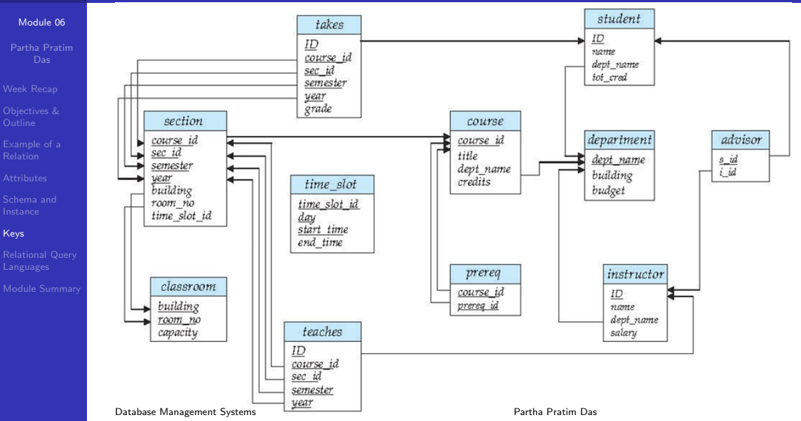
\includegraphics[height=0.8\textheight, width=\textwidth, keepaspectratio]{../Lecture 2.1_artifacts/image_000021_77d9c6955b12363d4815593e8422a1e8676257d51962ef788491ced4f30da518.png}
    \end{center}
\end{frame}

\section{Relational Query Languages}

\begin{frame}
  \vfill
  \centering
  \begin{beamercolorbox}[sep=8pt,center,shadow=true,rounded=true]{title}
    \usebeamerfont{title}Relational Query Languages\par%
  \end{beamercolorbox}
  \vfill
\end{frame}

\begin{frame}{Relational Query Languages}
    \textbf{Procedural viz-a-viz Non-procedural or Declarative Paradigms}
    \begin{itemize}
        \item \textbf{Procedural programming} requires that the programmer tell the computer \textit{what} to do
        \begin{itemize}
            \item That is, \textit{how} to get the output for the range of required inputs
            \item The programmer must know an appropriate algorithm
        \end{itemize}
        \item \textbf{Declarative programming} requires a more descriptive style
        \begin{itemize}
            \item The programmer must know what relationships hold between various entities
        \end{itemize}
    \end{itemize}
\end{frame}

\begin{frame}{Relational Query Languages (Cont..)}
    \textbf{Procedural vs. Non-procedural or Declarative Paradigms}
    \begin{itemize}
        \item Example: Square root of $n$
        \item \textbf{Procedural}
        \begin{enumerate}
            \item[a)] Guess $x_0$ (close to root of $n$)
            \item[b)] $i \leftarrow 0$
            \item[c)] $x_{i+1} \leftarrow (x_i + n / x_i) / 2$
            \item[d)] Repeat Step 2 if $|x_{i+1} - x_i| > \text{delta}$
        \end{enumerate}
        \item \textbf{Declarative}
        \begin{itemize}
            \item[$\triangleright$] Root of $n$ is $m$ such that $m^2 = n$
        \end{itemize}
    \end{itemize}
\end{frame}

\begin{frame}{Relational Query Languages (2)}
    \begin{itemize}
        \item `Pure' languages:
        \begin{itemize}
            \item Relational algebra
            \item Tuple relational calculus
            \item Domain relational calculus
        \end{itemize}
        \item The above 3 pure languages are equivalent in computing power
        \item We will concentrate on \textbf{relational algebra}
        \begin{itemize}
            \item Not Turing-machine equivalent
            \begin{itemize}
                \item[$\triangleright$] Not all algorithms can be expressed in RA
            \end{itemize}
            \item Consists of 6 basic operations
        \end{itemize}
    \end{itemize}
\end{frame}

\begin{frame}{Module Summary}
    \begin{itemize}
        \item Introduced the notion of attributes and their types
        \item Taken an overview of the mathematical structure of relational model -- schema and instance
        \item Introduced the notion of keys -- primary as well as foreign
    \end{itemize}
    \vspace{2em}
    \begin{center}
    \small \textit{Slides used in this presentation are borrowed from \url{http://db-book.com/} with kind permission of the authors.} \\
    \small \textit{Edited and new slides are marked with 'PPD'.}
    \end{center}
\end{frame}

\end{document}
